%提出するレポートの書式はこのtemplateファイルに沿って作成してください。
%特に表紙・概要の書式は変えないで下さい。

\documentclass[a4j]{jarticle}

\usepackage[dvipdfmx]{graphicx}
% \usepackage{epsbox}
\usepackage{url}
\usepackage{here}
\usepackage{ascmac}

\setlength{\headsep}{-5mm}
\setlength{\oddsidemargin}{0mm}
\setlength{\textwidth}{165mm}
\setlength{\textheight}{230mm}
\setlength{\footskip}{20mm}

\title{
\vspace{30mm}
{\bf 高知工科大学様}\\
\vspace{5mm}
大学掲示板(KUTBBS)\\
\vspace{5mm}
{\bf  内部設計書v1.0}
\vspace{90mm}
}
 \author{
\vspace{5mm}
グループ10 \\
\vspace{5mm}
Pathfinder \\
\vspace{5mm}
\vspace{10mm}
}

 \begin{document}
\maketitle
\newpage
\tableofcontents
\newpage


 \section{システム概要}
本システムは、学生が陥りやすいトラブルや、学生自身の学習における課題や悩みを自主的に解決するため の掲示板型のウェブアプリケーションである。 学生同士が問題をネット上でかつ匿名に解決できるようにするために開発するシステムが、本システムである。 利用する対象は、本校の学生である。また管理者は、本校の事務員を想定している。\\
 本システムは、メインシステムとして下記に示す「ユーザシステム」、「掲示板システム」、「管理者システム」 の 3 つを実装しており、各システムを構成するサブシステムも併せて以下に示す。
\begin{itemize}
\item 掲示板システム
	\begin{itemize}
	\item 掲示板サブシステム
	\item 検索サブシステム
	\item コレクトボタンサブシステム
	\item 通報サブシステム
	\item 通知サブシステム
	\end{itemize}
\item ユーザシステム
	\begin{itemize}
	\item アカウント登録サブシステム
	\item ログインサブシステム
	\item マイページサブシステム
	\item ブックマークサブシステム
	\item お知らせ表示サブシステム
	\end{itemize}
\item 管理者システム
	\begin{itemize}
	\item 管理者ログインサブシステム
	\item 子管理者管理サブシステム
	\item お知らせ編集サブシステム
	\item 掲示板編集サブシステム
	\item ユーザ管理サブシステム
	\end{itemize}
\end{itemize}
 \section{動作環境}
本システムの動作環境は以下の通りである。
\begin{itemize}
\item 動作環境
	\begin{itemize}
	\item CPU : ARM Cortex-A53 1GHz以上
	\item GPU : Broadcom VideoCore IV
	\item メモリ : 2GB以上
	\item ストレージ : 4GB eMMC / SDカードPIN
	\item OS
	\begin{itemize}
		\item Linux version 7
		\item ubuntu version 18.04
		\item MacOS
		\item Windowss7 , 8 , 10
		\item iOS 10.0
	\end{itemize}
	\item webサーバ : AWS EC2
	\item Appサーバ : Ruby on Rails version 5.1.4
	\item RDBMS : MySQL version 8.0
	\end{itemize}
\item 使用ブラウザ : GoogleChrome62.0 , Firefox version 57.0% , Safari11.0.1
\end{itemize}
\section{開発環境}
本システムの開発環境は以下の通りである。
\begin{itemize}
\item OS
	\begin{itemize}
		\item Linux version 7
		\item ubuntu version 18.04
		\item MacOS
		\item Windowss7 , 8 , 10
		\item iOS 10.0
	\end{itemize}
\item HTML : version5
\item 使用言語
	\begin{itemize}
	\item ruby version 2.4.2
	\item Ruby on Rails version 5.1.4
	\item CSS
	\item JavaScript
	\end{itemize}
\item サーバ :
\item データベース : MySQL version 8.0
\item webサーバ : AmazonWebServices
\end{itemize}
 \section{内部設計書作成方針}
\subsection{コーディング規約}
\subsubsection{命名規約}
\begin{itemize}
\item 変数名・メソッド名\\
‐ 小文字始まりとする\\
‐ 基本的に意味のある単語を使用する\\
‐
\end{itemize}
\begin{itemize}
\item 定数\\
‐ 全て大文字を使用する\\
\end{itemize}
\begin{itemize}
\item クラス名・構造体名\\
‐ 変数名・メソッド名を同様に意味のある単語を使用する\\
‐ 大文字始まりとする\\
‐ 複数の単語を組み合わせる際は先頭文字を大文字で表記する\\
\end{itemize}
\subsubsection{コーディングスタイル}
\begin{itemize}
\item インデント\\
‐ インデントにはタブを使用する(半角スペース4文字)
\end{itemize}
\begin{itemize}
\item 括弧\\
‐ 中括弧は改行して始める\\
‐ 小括弧の前後にはスペースを使用しない
\end{itemize}
\begin{itemize}
\item 演算子\\
‐ 演算子の前後には半角スペースを一文字使用する
\end{itemize}
\subsection{設計書作成環境}
内部設計書の作成環境は,表\ref{tab:creating_environment}に示します。
\begin{table}[htb]
\caption{内部設計書の作成環境環境}
\begin{center}
  \begin{tabular}{|c|c|} \hline
    組版処理システム & LATEX,dvpdfmx\\ \hline
   文字コード &  UTF-8\\ \hline
    改行コード & LF(0x0A)  \\ \hline
  \end{tabular}
\label{tab:creating_environment}
\end{center}
\end{table}
\subsection{サーバ環境}
本システムを利用するためにはAmazon Web Services(AWS) の EC2 インスタンスを用いて実現します.サーバ環境は表\ref{tab:server_environment}に示します。
\begin{table}[htb]
\caption{サーバ側の動作環境}
\begin{center}
  \begin{tabular}{|c|c|} \hline
    対応OS & Ruby on Rails \\ \hline
   vCPU & 1\\ \hline
    メモリ(GiB) & 1  \\ \hline
    ストレージ & 30GB \\ \hline
  \end{tabular}
\label{tab:server_environment}
\end{center}
\end{table}
\section{データベース設計}
本章では本システムにおけるデータベースMySQLについてを示す。

\subsection{データテーブル構成}
本小節ではデータテーブルの構成をER図を用いて示す。


\begin{figure}[H]
\begin{center}
\resizebox{10cm}{!}{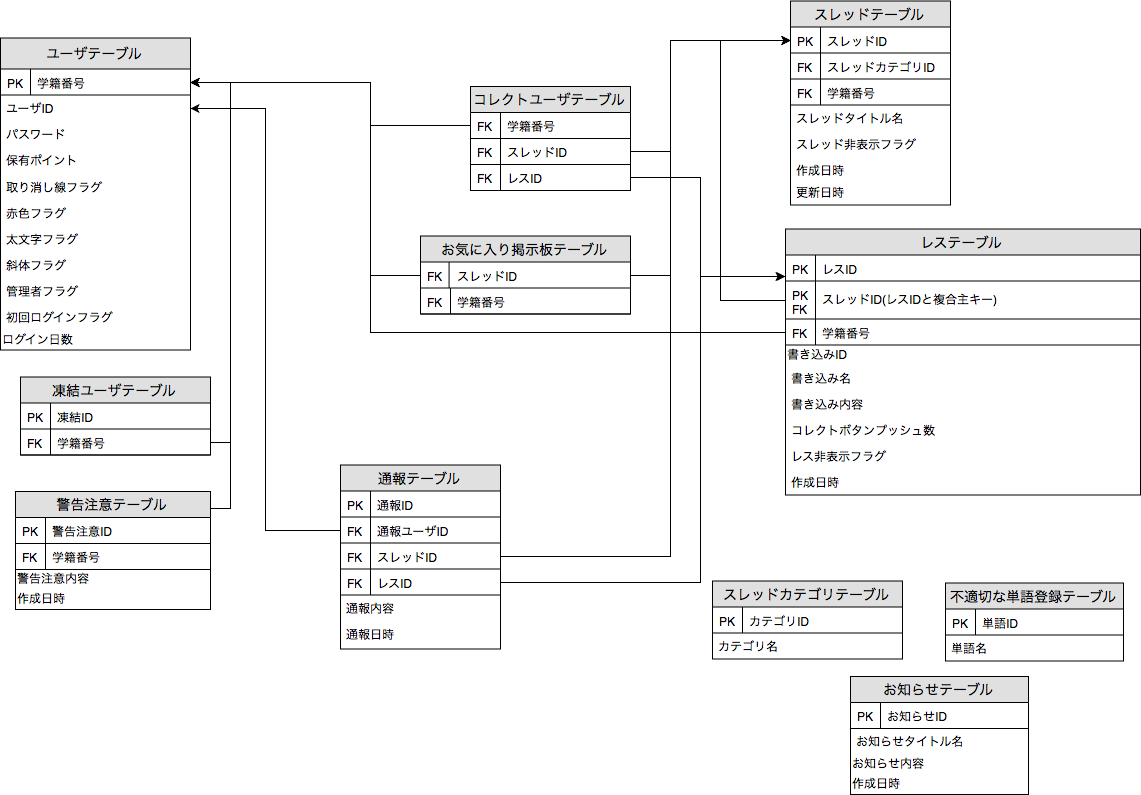
\includegraphics{date-ER1.png}}
\caption{ER図}
\label{}
\end{center}
\end{figure}
\newpage

\subsection{テーブル設計}
本小節ではデータベース構成するテーブルについて示す。また、各カラムについても詳細も示す。

\subsubsection{ユーザテーブル(user)}
ユーザテーブルではユーザに関する情報を管理する。このテーブルの詳細は表\ref{tab:user} に示す。
\begin{table}[h]

  \caption{ユーザテーブル}
  \begin{center}
    \footnotesize
    \begin{tabular}{|l|l|l|c|c|l|l|} \hline

      \multicolumn{1}{|c|}{論理名}&\multicolumn{1}{|c|}{物理名}&\multicolumn{1}{|c|}{データ型}&精度&NULL&\multicolumn{1}{|c|}{オプション}&\multicolumn{1}{|c|}{PK/FK:mode}\\\hline \hline
      学籍番号&student\verb|_|id&char&7&×&-&\multicolumn{1}{|l|}{PK} \\\hline
      ユーザID&user\verb|_|id&varchar&20&×&-&- \\ \hline
      パスワード&password&varchar&20&×&-&- \\ \hline
      保有ポイント&now\verb|_|point&int&4&×&-&- \\ \hline
      取り消しフラグ&cancel\verb|_|flag&int&1&×&-&- \\ \hline
      赤色フラグ&color\verb|_|flag&int&1&×&-&- \\ \hline
      斜体フラグ&diagonal\verb|_|flag&int&1&×&-&- \\ \hline
      太文字フラグ&bold\verb|_|letters\verb|_|flag&int&1&×&-&- \\ \hline
      管理者フラグ&administrator\verb|_|flag&int&1&○&-&- \\ \hline
      初回ログインフラグ&first\verb|_|login\verb|_|flag&int&1&×&-&- \\ \hline
      ログイン日数&count\verb|_|login&int&4&×&-&-\\ \hline 
    \end{tabular}
    \label{tab:user}
  \end{center}
\end{table}

\begin{itemize}
\item 学籍番号\\
  ユーザの学籍番号を示す値であり、自テーブルの主キーである。NULL値は含まない。値は固定7文字の半角英数字にて構成される。\\
\item ユーザID\\
  ユーザを識別するためのIDを示す値である。NULL値は含まない。値は20文字以下の半角英数字にて構成される。
\item パスワード\\
  ユーザを識別するためのパスワードを示す値である。NULL値は含まない。値は20文字以下の半角英数字にて構成される。\\
\item 保有ポイント\\
  ユーザがログインした日数とコレクトボタンを10回以上押されたことで獲得したポイントを示す値である。NULL値は含まない。4桁(0001から9999)の数値にて構成される。

\item 取り消しフラグ\\
  拡張機能の1つであり、取り消し線を付与することを示す値である。NULL値は含まない。値は1桁の0(OFF)、1(ON)の数値にて構成される。\\
  
\item 赤色フラグ\\
  拡張機能の1つであり、赤色を付与することを示す値である。NULL値は含まない。値は1桁の0(OFF)、1(ON)の数値にて構成される。\\
\item 斜体フラグ\\
  拡張機能の1つであり、斜体を付与することを示す値である。NULL値は含まない。値は1桁の0(OFF)、1(ON)の数値にて構成される。\\

\item 太文字フラグ\\
  拡張機能の1つであり、太文字を付与することを示す値である。NULL値は含まない。値は1桁の0(OFF)、1(ON)の数値にて構成される。\\

\item 管理者フラグ\\
  親管理者と子管理者を識別することを示す値である。値は1桁の0(子管理者)、1(親管理者)の数値にて構成される。\\
\item 初回ログインフラグ\\
  初回ログインを識別することを示す値である。NULL値は含まない。値は1桁の0(OFF)、1(ON)の数値にて構成される。
  
\item ログイン日数\\
  ユーザがログインをした日数を記録することを示す値である。NULL値は含まない。値は4桁(0001から9999)の数値にて構築される。
  
   \end{itemize}
\newpage
  \subsubsection{スレッドテーブル(thread)}
  スレッドテーブルではスレッドに関する情報を管理する。このテーブルの詳細は表\ref{tab:thread} に示す。
  \begin{table}[h]
    \caption{スレッドテーブル}
    \begin{center}
      %\fontsize{6.5pt}{30pt}\selectfont
      \footnotesize
      \begin{tabular}{|l|l|l|c|c|l|l|} \hline
        \multicolumn{1}{|c|}{論理名}&\multicolumn{1}{|c|}{物理名}&\multicolumn{1}{|c|}{データ型}&精度&NULL&\multicolumn{1}{|c|}{オプション}&\multicolumn{1}{|c|}{PK/FK:mode}\\\hline \hline
        スレッドID&thread\verb|_|id&int&5&×&\begin{tabular}{l}unsigned zerofill\\auto\verb|_|increment\end{tabular}&\multicolumn{1}{|l|}{PK} \\\hline
          スレッドカテゴリID&thread\verb|_|category\verb|_|id&int&3&×&\begin{tabular}{l}unsigned zerofill\\auto\verb|_|increment\end{tabular}&FK:thread\verb|_|category \\ \hline
            学籍番号&student\verb|_|id&char&7&×&-&\multicolumn{1}{|l|}{FK:user} \\\hline
            スレッドタイトル名&thread\verb|_|category\verb|_|name&varchar&50&×&-&- \\ \hline
            スレッド非表示フラグ&thread\verb|_|hide\verb|_|flag&int&1&×&-&- \\ \hline
            作成日時&created\verb|_|at&timestamp&-&×&default current\verb|_|timestamp&- \\ \hline
            更新日時&updated\verb|_|at&timestamp&-&×&\begin{tabular}{l}default current\verb|_|timestamp on \\update current\verb|_|timestamp\end{tabular}&- \\ \hline
      \end{tabular}
      
      \label{tab:thread}
    \end{center}
  \end{table}
  \begin{itemize}  
  \item スレッドID\\
    自テーブルの主キーである。NULL値は含まない。値は5桁(00001から99999)の数値にて構成され自動追加される。\\

  \item スレッドカテゴリID\\
    スレッドカテゴリテーブルを参照する際の外部キーである。NULL値は含まない。値は3桁(001から999)の数値にて構成され自動追加される。\\
    
  \item 学籍番号\\
    ユーザテーブルを参照する際の外部キーである。NULL値は含まない。固定7文字の半角英数字にて構成される。\\
    
  \item スレッドタイトル名\\
    スレッドタイトルを示す値である。NULL値は含まない。値は50文字以下の文字列にて構成される。\\
  \item スレッド非表示フラグ\\
    管理者の操作権限でスレッドを非表示を示す値である。NULL値は含まない。値は1桁の数値で0(OFF)、1(ON)の数値にて構成される。\\
    例としてスレッド非表示フラグを1にした場合、ユーザ側からはスレッドが非表示になる。
  \item 作成日時\\
    レコードを作成した日付・時刻を示す値である。NULL値は含まない。レコードが作成されるたびに自動追加を行う。
  \item 更新日時\\
    レコードを更新した日付・時刻を示す値である。NULL値は含まない。レコードが更新されるたびに自動更新を行う。
  \end{itemize}
  \subsubsection{レステーブル(res)}
  レステーブルではレスに関する情報を管理する。このテーブルの詳細は表\ref{tab:ress} に示す。
  \begin{table}[h]
    \caption{レステーブル}
    \begin{center}
      %\fontsize{6.5pt}{30pt}\selectfont
      \footnotesize
      \begin{tabular}{|l|l|l|c|c|l|l|} \hline
        \multicolumn{1}{|c|}{論理名}&\multicolumn{1}{|c|}{物理名}&\multicolumn{1}{|c|}{データ型}&精度&NULL&\multicolumn{1}{|c|}{オプション}&\multicolumn{1}{|c|}{PK/FK:mode}\\\hline \hline
        レスID&res\verb|_|id&int&4&×&\begin{tabular}{l}unsigned zerofill\\auto\verb|_|increment\end{tabular}&PK \\\hline
          スレッドID&thread\verb|_|id&int&5&×&\begin{tabular}{l}unsigned zerofill\\auto\verb|_|increment\end{tabular}&\begin{tabular}{l}PK(res複合)\\FK:thread\end{tabular}\\\hline
              学籍番号&student\verb|_|id&char&7&×&-&\multicolumn{1}{|l|}{FK:user} \\\hline
              書き込みID&write\verb|_|id&char&8&×&-&-\\ \hline 
              書き込み名&write\verb|_|name&varchar&15&×&-&- \\ \hline
              書き込み内容&write\verb|_|content&varchar&200&×&-&- \\ \hline
              コレクトプッシュ数&collect\verb|_|push\verb|_|count&int&4&×&-&- \\ \hline
              書き込みID&write\verb|_|id&char&8&×&-&-\\ \hline 
              レス非表示フラグ&res\verb|_|hide\verb|_|flag&int&1&×&-&- \\ \hline
              作成日時&created\verb|_|at&timestamp&-&×&default current\verb|_|timestamp&- \\ \hline
      \end{tabular}
      
      \label{tab:ress}
    \end{center}
  \end{table}
  
  \begin{itemize}
  \item レスID\\
    自テーブルの主キーである。NULL値は含まない。値は4桁(0001から9999)の数値にて構成され自動追加される。
  \item スレッドID\\
    スレッドテーブルを参照する際の外部キーであり、スレIDとの複合主キーである。NULL値は含まない。値は5桁(00001から99999)の数値にて構成され自動追加される。
  \item 学籍番号\\
    ユーザテーブルを参照する際の外部キーである。NULL値は含まない。固定7文字の半角英数字にて構成される。\\
  \item 書き込みID\\
    ユーザが書き込みを行う際に表示するIDを示す値である。NULL値は含まない。値は固定8文字の半角英数字にて構成される。\\   
  \item 書き込み名\\
    書き込みを行う際に表示する名前を示す値である。NULL値は含まない。値は15文字以下の文字列にて構成される。\\
  \item 書き込み内容\\
    書き込み内容を示す値である。NULL値は含まない。値は200文字以下の文字列にて構成される。\\
  \item コレクトボタンプッシュ数\\
    レスに対してコレクトボタンが押された回数を示す値である。NULL値は含まない。値は4桁(0001から9999)の数値にて構成される。\\
  \item レス非表示フラグ\\
    管理者の操作権限でレスを非表示を示す値である。NULL値は含まない。値は1桁の数値で0(OFF)、1(ON)の数値にて構成される。\\
    例としてレス非表示フラグを1にした場合、ユーザ側からはレスが非表示になる。
    
  \item 作成日時\\
    レコードを作成した日付・時刻を示す値である。NULL値は含まない。レコードが作成されるたびに自動追加される。    
  \end{itemize}

  \subsubsection{スレッドカテゴリテーブル(thread\_category)}
  スレッドカテゴリテーブルは各カテゴリごとに分けられたスレッドの情報を管理する。このテーブルの詳細は表\ref{tab:thread_category} に示す。
  \begin{table}[h]
    \caption{スレッドカテゴリテーブル}
    \begin{center}
      %\fontsize{6.5pt}{30pt}\selectfont
      \footnotesize
      \begin{tabular}{|l|l|l|c|c|l|l|} \hline
        \multicolumn{1}{|c|}{論理名}&\multicolumn{1}{|c|}{物理名}&\multicolumn{1}{|c|}{データ型}&精度&NULL&\multicolumn{1}{|c|}{オプション}&\multicolumn{1}{|c|}{PK/FK:mode}\\\hline \hline
        カテゴリID&category\verb|_|no&int&3&×&\begin{tabular}{l}unsigned zerofill\\auto\verb|_|increment\end{tabular}&PK\\ \hline
          カテゴリ名&category\verb|_|name&varchar&15&×&-&-\\\hline
      \end{tabular}
      \label{tab:thread_category}
    \end{center}
  \end{table}
  
  \begin{itemize}
  \item カテゴリID\\
    自テーブルの主キーである。NULL値は含まない。値は3桁(001から999)の数値にて構築され自動追加される。
  \item カテゴリ名\\
    カテゴリの名前を示す値である。NULL値は含まない。値は15文字以下の文字列にて構成される。\\
    
  \end{itemize}

  \subsubsection{お気に入り掲示板テーブル(favorite\_bbs)}
  お気入り掲示板テーブルではブックマークとして登録したスレッド情報を管理する。このテーブルの詳細は表\ref{tab:favorite_bbs} に示す。
  \begin{table}[h]
    \caption{お気に入り掲示板テーブル}
    \begin{center}
      %\fontsize{6.5pt}{30pt}\selectfont
      \footnotesize
      \begin{tabular}{|l|l|l|c|c|l|l|} \hline
        \multicolumn{1}{|c|}{論理名}&\multicolumn{1}{|c|}{物理名}&\multicolumn{1}{|c|}{データ型}&精度&NULL&\multicolumn{1}{|c|}{オプション}&\multicolumn{1}{|c|}{PK/FK:mode}\\\hline \hline
        学籍番号&student\verb|_|id&char&7&×&-&\multicolumn{1}{|l|}{FK:user} \\\hline
        スレッドID&thread\verb|_|id&int&5&×&\begin{tabular}{l}unsigned zerofill\\auto\verb|_|increment\end{tabular}&FK:thread\\\hline
      \end{tabular}
      \label{tab:favorite_bbs}
    \end{center}
  \end{table}
  
  \begin{itemize}
  \item 学籍番号\\
    ユーザテーブルを参照する際の外部キーである。NULL値は含まない。固定7文字の半角英数字にて構成される。\\
  \item スレッドID\\
    スレッドテーブルを参照する際の外部キーである。NULL値は含まない。値は5桁(00001から99999)の数値にて構築され自動追加される。
  \end{itemize}
  
  
  
  \subsubsection{コレクトユーザテーブル(collect\_user)}
  コレクトユーザテーブルではコレクトボタンを押されたことに関する情報を管理する。このテーブルの詳細は表 \ref{tab:collect_user} に示す。
  \begin{table}[h]
    \caption{コレクトユーザテーブル}
    \begin{center}
      %\fontsize{6.5pt}{30pt}\selectfont
      \footnotesize
      \begin{tabular}{|l|l|l|c|c|l|l|} \hline
        \multicolumn{1}{|c|}{論理名}&\multicolumn{1}{|c|}{物理名}&\multicolumn{1}{|c|}{データ型}&精度&NULL&\multicolumn{1}{|c|}{オプション}&\multicolumn{1}{|c|}{PK/FK:mode}\\\hline \hline
        学籍番号&student\verb|_|id&char&7&×&-&\multicolumn{1}{|l|}{FK:user} \\\hline
        スレッドID&thread\verb|_|id&int&5&×&\begin{tabular}{l}unsigned zerofill\\auto\verb|_|increment\end{tabular}&FK:thread\\\hline
          レスID&res\verb|_|no&int&4&×&\begin{tabular}{l}unsigned zerofill\\auto\verb|_|increment\end{tabular}&FK:res \\\hline
      \end{tabular}
      \label{tab:collect_user}
    \end{center}
  \end{table}

  \begin{itemize}
  \item 学籍番号\\
    ユーザテーブルを参照する際の外部キーである。NULL値は含まない。固定7文字の半角英数字にて構成される。\\
  \item スレッドID\\
    スレッドテーブルを参照する際の外部キーである。NULL値は含まない。値は5桁(00001から99999)の数値にて構成され自動追加される。
  \item レスID\\
    レステーブルを参照する際の外部キーである。NULL値は含まない。値は4桁(0001から9999)の数値にて構成され自動追加される。
  \end{itemize}

  \subsubsection{不適切な単語登録テーブル(inadequacy\_word)}
  不適切な単語登録テーブルでは管理者が誹謗中傷や公序良俗に違反していると考えられる単語を登録した情報を管理する。このテーブルの詳細は表 \ref{tab:inadequacy_word} に示す。
  \begin{table}[h]
    \caption{不適切な単語登録テーブル}
    \begin{center}
      %\fontsize{6.5pt}{30pt}\selectfont
      \footnotesize
      \begin{tabular}{|l|l|l|c|c|l|l|} \hline
        \multicolumn{1}{|c|}{論理名}&\multicolumn{1}{|c|}{物理名}&\multicolumn{1}{|c|}{データ型}&精度&NULL&\multicolumn{1}{|c|}{オプション}&\multicolumn{1}{|c|}{PK/FK:mode}\\\hline \hline
        単語ID&word\verb|_|id&int&5&×&\begin{tabular}{l}unsigned zerofill\\auto\verb|_|increment\end{tabular}&PK\\\hline
          単語名&word\verb|_|name&varchar&200&×&-&- \\\hline
      \end{tabular}
      \label{tab:inadequacy_word}
    \end{center}
  \end{table}
  
  \begin{itemize}
  \item 単語ID\\
    自テーブルの主キーである。NULL値は含まない。値は5桁(00001から99999)の数値にて構成され自動追加される。
  \item 単語名\\
    管理者の操作権限で登録した単語を示す値である。NULL値は含まない。値は200文字以下の文字列にて構成される。
  \end{itemize}

  
  \subsubsection{通報テーブル(report)}
  通報テーブルではユーザが誹謗中傷や公序良俗に違反するなどの不適切な内容であると判断したスレッドまたはレスを管理者に通報した時の情報を管理する。また、通報した内容の情報も管理する。このテーブルの詳細は表 \ref{tab:report} に示す。
  \begin{table}[h]
    \caption{通報テーブル}
    \begin{center}
      %\fontsize{6.5pt}{30pt}\selectfont
      \footnotesize
      \begin{tabular}{|l|l|l|c|c|l|l|} \hline
        \multicolumn{1}{|c|}{論理名}&\multicolumn{1}{|c|}{物理名}&\multicolumn{1}{|c|}{データ型}&精度&NULL&\multicolumn{1}{|c|}{オプション}&\multicolumn{1}{|c|}{PK/FK:mode}\\\hline \hline
        通報ID&report\verb|_|id&int&5&×&\begin{tabular}{l}unsigned zerofill\\auto\verb|_|increment\end{tabular}&PK\\\hline
          通報ユーザID&report\verb|_|user\verb|_|id&varchar&20&×&-&FK:user \\ \hline
          スレッドID&thread\verb|_|id&int&5&×&\begin{tabular}{l}unsigned zerofill\\auto\verb|_|increment\end{tabular}&FK:thread\\\hline
            レスID&res\verb|_|id&int&4&×&\begin{tabular}{l}unsigned zerofill\\auto\verb|_|increment\end{tabular}&FK:res \\\hline
              通報内容&report\verb|_|content&varchar&200&×&-&-\\ \hline
              通報日時&report\verb|_|at&timestamp&-&×&default current\verb|_|timestamp&- \\ \hline
      \end{tabular}
      \label{tab:report}
    \end{center}
  \end{table}
  
  \begin{itemize}
  \item 通報ID\\
    自テーブルの主キーである。NULL値は含まない。値は5桁(00001から99999)の数値にて構成され自動追加される。
  \item 通報ユーザID\\
    ユーザテーブルを参照する際の外部キーである。NULL値は含まない。値は20文字以下の半角英数字にて構成される。\\

  \item スレッドID\\
    スレッドテーブルを参照する際の外部キーである。NULL値は含まない。値は5桁(00001から99999)の数値にて構成され自動追加される。
  \item レスID\\
    レステーブルを参照する際の外部キーである。NULL値は含まない。値は4桁(0001から9999)の数値にて構成され自動追加される。
  \item 通報内容\\
    通報内容を示す値である。NULL値は含まない。値は200文字以下の文字列にて構成される。\\
    
  \item 通報日時\\
    レコードを作成した日付・時刻を示す値である。NULL値は含まない。レコードが作成されるたびに自動追加を行う。
  \end{itemize}
  
  \subsubsection{凍結ユーザテーブル(suspend)}
  凍結ユーザテーブルでは迷惑行為が改善されないユーザのアカウントを凍結した情報を管理する。このテーブルの詳細は表 \ref{tab:suspend} に示す。
  
  \begin{table}[h]
    \caption{凍結ユーザテーブル}
    \begin{center}
      \fontsize{6.5pt}{30pt}\selectfont
      \footnotesize
      \begin{tabular}{|l|l|l|c|c|l|l|} \hline
        \multicolumn{1}{|c|}{論理名}&\multicolumn{1}{|c|}{物理名}&\multicolumn{1}{|c|}{データ型}&精度&NULL&\multicolumn{1}{|c|}{オプション}&\multicolumn{1}{|c|}{PK/FK:mode}\\\hline \hline
        凍結ID&suspend\verb|_|id&int&4&×&\begin{tabular}{l}unsigned zerofill\\auto\verb|_|increment\end{tabular}&PK\\\hline
          学籍番号&student\verb|_|id&char&7&×&-&\multicolumn{1}{|l|}{FK:user} \\\hline
      \end{tabular}
      \label{tab:suspend}
    \end{center}
  \end{table}
  
  \begin{itemize}
  \item 凍結ID\\
    自テーブルの主キーである。NULL値は含まない。値は4桁(0001から9999)の数値にて構成され自動追加される。
  \item 学籍番号\\
    ユーザテーブルを参照する際の外部キーである。。NULL値は含まない。値は固定7文字の半角英数字にて構成される。\\
  \end{itemize}
  
  \subsubsection{お知らせテーブル(news)}
  お知らせテーブルではお知らせに関する情報を管理する。このテーブルの詳細は表 \ref{tab:news} に示す。
  \begin{table}[h]
    \caption{お知らせテーブル}
    \begin{center}
      \fontsize{6.5pt}{30pt}\selectfont
      \footnotesize
      \begin{tabular}{|l|l|l|c|c|l|l|} \hline
        \multicolumn{1}{|c|}{論理名}&\multicolumn{1}{|c|}{物理名}&\multicolumn{1}{|c|}{データ型}&精度&NULL&\multicolumn{1}{|c|}{オプション}&\multicolumn{1}{|c|}{PK/FK:mode}\\\hline \hline
        お知らせID&news\verb|_|id&int&5&×&\begin{tabular}{l}unsigned zerofill\\auto\verb|_|increment\end{tabular}&PK\\\hline
          お知らせタイトル名&news\verb|_|title&varchar&50&×&-&-\\\hline
          お知らせ内容&news\verb|_|title&varchar&400&×&-&-\\\hline
          作成日時&created\verb|_|at&timestamp&-&×&default current\verb|_|timestamp&- \\ \hline
          
      \end{tabular}
      \label{tab:news}
    \end{center}
  \end{table}
  
  \begin{itemize}
  \item お知らせID\\
    自テーブルの主キーである。NULL値は含まない。値は5桁(00001から99999)の数値にて構成され自動追加される。
  \item お知らせタイトル名\\
    お知らせタイトルを示す値である。NULL値は含まない。値は50文字以下の文字列にて構成される。
  \item お知らせ内容\\
    お知らせ内容を示す値である。NULL値は含まない。値は400文字以下の文字列にて構成される。\\

  \item 作成日時\\
    レコードを作成した日付・時刻を示す値である。NULL値は含まない。レコードが作成されるたびに自動追加を行う。    
  \end{itemize}
  \subsubsection{警告注意テーブル(warned\_caution)}
  警告テーブルでは管理者がユーザに対しての警告・注意喚起に関する情報を管理する。このテーブルの詳細は表 \ref{tab:warned_caution} に示す。
  \begin{table}[h]
    \caption{警告注意テーブル}
    \begin{center}
      \fontsize{6.5pt}{30pt}\selectfont
      \footnotesize
      \begin{tabular}{|l|l|l|c|c|l|l|} \hline
        \multicolumn{1}{|c|}{論理名}&\multicolumn{1}{|c|}{物理名}&\multicolumn{1}{|c|}{データ型}&精度&NULL&\multicolumn{1}{|c|}{オプション}&\multicolumn{1}{|c|}{PK/FK:mode}\\\hline \hline
        警告注意ID&warned\verb|_|caution\verb|_|id&int&4&×&\begin{tabular}{l}unsigned zerofill\\auto\verb|_|increment\end{tabular}&PK\\\hline
          学籍番号&student\verb|_|id&char&7&×&-&\multicolumn{1}{|l|}{FK:user} \\\hline

          警告注意タイトル名&warned\verb|_|caution\verb|_|title&varchar&50&×&-&-\\\hline
          警告注意内容&warned\verb|_|caution\verb|_|title&varchar&400&×&-&-\\\hline
          作成日時&created\verb|_|at&timestamp&-&×&default current\verb|_|timestamp&- \\ \hline
          
      \end{tabular}
      \label{tab:warned_caution}
    \end{center}
  \end{table}

  \begin{itemize}
  \item 警告注意ID\\
    自テーブルの主キーである。NULL値は含まない。値は4桁(0001から9999)の数値にて構成され自動追加される。
  \item 学籍番号\\
    ユーザテーブルを参照する際の外部キーである。NULL値は含まない。値は固定7文字の半角英数字にて構成される。\\
    
  \item 警告注意タイトル名\\
    警告注意タイトルを示す値である。NULL値は含まない。値は50文字以下の文字列にて構成される。
  \item 警告注意内容\\
    警告注意内容を示す値である。NULL値は含まない。値は400文字以下の文字列にて構成される。\\
    
  \item 作成日時\\
    レコードを作成した日付・時刻を示す値である。NULL値は含まない。レコードが作成されるたびに自動追加を行う。
  \end{itemize}

\section{ルーティング及びMVC一覧}
この章では、Railsの規約に従ったURL規則を示す。また、HTTPメソッドとURLによって呼び出されるControllerとActionを示す。さらに、View及びModelも示す。
\newpage
\subsection{ルーティング一覧}
以下の表は、Railsの規則に従ったURL規則の表である。また、ControllerとそのActionについても示す。



\begin{table}[htb]
  \caption{ルーティング一覧}
  \centering
  \begin{tabular}{|l|l|l||l|} \hline
    No.&   URL 						&METHOD & Controller\#Action \\ \hline \hline
	 1&	/Login  					 	& GET      & sessions\#new       \\
       2&  	~		         			& POST    & sessions\#create	\\
	 3&	/Logout   				      &DELETE   &sessions\#destroy	\\
	 4&	/passwords/:id					&GET	  &passwords\#new    \\
	 5 & /passwords/:id					&PATCH	  &passwords\#change \\
	 6&	/home   						& GET 	   &home\_pages/\#home    \\
       7&	/home   						& PATCH 	   &home\_pages/\#threads\_hide \\
	 8&	/users/:id     					&  GET  	    &  users\#show       \\
	 9&	/users/:id     					 & PATCH   &  users\#update       \\
	10&	/results/:title         			& GET   	    & results\#search      \\
	11& /results/:title/categories/:id		&GET		& categories\#search	\\
	12&	/informations/:id				  & GET       & informations\#show      \\
	13&	/categories/:id    		   		 &   GET      & categories\#index    \\
	14&	/threads/new      	 	  		 &  GET      &  threads\#new         \\
	15&/threads/check      		       &  GET      & threads\#check       \\
	16&/threads                   		       &  POST    &threads\#create      \\
	17&/threads/:id/report\_new   		&   GET      &threads\#report\_new  \\
	18&	/threads/check               		&   GET      & threads\#check       \\
	19&	/threads                      		 & POST     & threads\#create     \\
	20&	/threads/:id/contents      		 &    GET    & contents\#bbs        \\
	21&	/threads/:id/contents/check 	&     GET    &  contents\#check   \\
	22&	/threads/:id/contents          	 &    POST  & contents\#write     \\
	23&	/threads/:id/contents          	 &    PATCH  & contents\#responses\_hide     \\
	24&	/threads/:id/contents/:id/report	 &    GET    & contents\#report    \\
	25&	/threads/:id/contents/:id/check   &   GET    &  contents\#check      \\
	26&	/threads/:id/contents            	 &   POST   & contents\#report\_create \\ \hline

\end{tabular}

\end{table}

\subsection{ルーティング(管理者側)一覧}
\underline{\bf( v2でユーザ側と管理者側を統合・修正します。)}\\
呼び出されたURLとHTTPメソッドによってRailsで呼び出すControllerのアクションを定義する。
\begin{table}[H]
  \centering
  \caption{ルーティング(管理者側)一覧}
  \begin{tabular}{|c|l|l|l|}\hline
    No. & URL & METHOD & Controller\#Action \\ \hline \hline
    1 & admins/login & GET & admins\_session \\
    2 & admins/login & POST & admins\_session\#login \\
    3 & admins/logout & POST & admins\_session\#logout \\ \hline
    4 & admins/top & GET & admins\_top\#home \\ \hline
    5 & admins/ng\_word & GET & ng\_word\#home \\
    6 & admins/ng\_word/create & POST & ng\_word\#create \\
    7 & admins/ng\_word/destroy & DELETE & ng\_word\#destroy \\ \hline
    8 & admins/manage & GET & manage\#home \\
    9 & admins/manage/signup & GET & manage\#signup \\
    10 & admins/manage/create & POST & manage\#create \\
    11 & admins/manage/ok & GET & manage\#ok \\
    12 & admins/manage/destroy\_check & GET & manage\#destroy\_check \\
    13 & admins/manage/destroy & DELETE & manage\#destroy \\ \hline
    14 & admins/manage\_user & GET & manage\_user\#home \\
    15 & admins/manege\_user/signup & GET & manage\_user\#user\_signup \\
    16 & admins/manage\_user/create & POST & manage\_user\#user\_create \\
    17 & admins/manage\_user/search & GET & manage\_user\#search \\
    18 & admins/manage\_user/:id & GET & manage\_user\#info \\
    19 & admins/manage\_user/warning\_edit & GET & manage\_user\#warning\_edit \\
    20 & admins/manage\_user/warning\_check & GET & manage\_user\#warning\_check \\
    21 & admins/manage\_user/warning\_send & POST & manage\_user\#warning\_send \\
    22 & admins/manage\_user/ban & PATCH & manage\_user\#ban \\ \hline
    23 & admins/announce & GET & announce\#edit \\
    24 & admins/announce\_check & GET & announce\#check \\
    25 & admins/announce\_send & POST & announce\#send \\ \hline
    26 & admins/report & GET & report\#home \\
    27 & admins/report/hide & PATCH & report\#hide \\ \hline
  \end{tabular}
\end{table}



\subsection{Controller}
\subsubsection{sessions\_controller.rb}
\noindent 名称:セッション情報処理	\newline
処理: \newline
-new:ログインフォームであるsessions\_new.html.erbを表示させる。\newline
-create:ユーザのIDとパスワードで認証を行い、認証されるとそのユーザのセッションを作成する。セッションを作成したユーザによって、以下のルーティングにリクエストを行う。\newline
ユーザが管理者:/adminに対してGETメソッドでルーティングにリクエストを行う。\newline
ユーザが一般ユーザ:/homeに対してGETメソッドでルーティングにリクエストを行う。また、そのユーザが初回ログインの場合は、/passwordsにGETメソットでルーティングにリクエストを行う。なお、認証が失敗した場合は再度/Loginに対してGETメソッドでルーティングを行う。\newline
-destroy:作成したユーザのセッションを破棄する。

\subsubsection{passwords\_controller.rb}
\noindent 名称:パスワード変更処理	\newline
処理:\newline
-new:初回ログインを行なった該当するユーザに対して、パスワード変更用フォームであるpasswords\_new.html.erbを表示させる。\newline
-change:あらかじめ登録されていたユーザのパスワード情報を、変更用フォームから入力された新しいパスワードに更新する。更新後、/homeに対してGETメソッドでルーティングにリクエストする。

%「該当する」という文言は、ユーザのidやスレッドのtitle等、DB上からなんらかの(一意な)属性の値を取得する処理が存在することを意味する



\subsubsection{home\_controller.rb}
\noindent 名称:ホーム画面処理 \newline
処理:\newline
-home:ホーム画面であるhome.html.erbを表示する。スレッドタイトル入力テキストボックスに検索したいスレッドタイトルを入力し、検索ボタンを押すと、/results/:idにGETメソッドでルーティングにリクエストを行う。お知らせを押すと、/infomations/:idにGETメソッドでルーティングを行う。マイページボタンを押すと、/user/:idにGETメソッドでルーティングを行う。\newline
%管理者が推すと管理者ページへ戻る?
-threads\_hide:不適切なスレッドを非表示化する。この処理は、管理者以外行うことはできない(非表示化ボタン自体が存在しない)。このアクションを行うと、/homeに対してPATCHメソッドでルーティングにリクエストする。



\subsubsection{users\_controller.rb}
\noindent 名称:マイページ画面処理 \newline
処理:\newline
-show:マイページ画面であるshow.html.erbを表示する。\newline
-update:拡張機能を開放する(Userテーブルにおけるユーザの各種拡張フラグを1に更新する)アクションである。解放後、/user/:idにPATCHメソッドでルーティングにリクエストする。


\subsubsection{results\_controller.rb}
\noindent 名称:スレッドタイトル検索処理 \newline
処理:\newline
-search:スレッドタイトル検索機能の処理を行うアクションである。検索を行い、該当するスレッドを取得した後は、そのスレッドを一覧として表示する(これがsearch.html.erbとなる)。表示されたスレッドタイトルを押すと、/threads/:id/contentsにGETメソッドでルーティングをリクエストする。\newline

\subsubsection{results\_categories\_controller.rb}
\noindent 名称:カテゴリ別スレッドタイトル検索処理 \newline
処理:\newline
-search:スレッドタイトル検索機能の処理を行うアクションである。先ほど述べたスレッドタイトル検索処理とほとんど同じであるが、スレッドタイトル以外にも、該当するカテゴリであるかどうかを条件として検索を行う処理である。検索条件以外の処理に違いは存在しない。\newline



\subsubsection{infomations\_controller.rb}
\noindent 名称:お知らせ画面処理 \newline
処理:\newline
-show:お知らせ詳細画面であるshow.html.erbを表示する。\newline



\subsubsection{categories\_controller.rb}
\noindent 名称:カテゴリ別トップ画面処理 \newline
処理:\newline
-new:カテゴリ別トップ画面であるcategories.html.erbを表示する。この画面もトップ画面同様、スレッドタイトル入力テキストボックスが存在しているがこちらから検索を行うと、/results/:title/categories/:idにGETメソッドでルーティングをリクエストする。マイページに遷移するボタンの処理は、トップ画面と同様である。また、スレッドタイトルを押した場合は、/threads/:id/contentsにGETメソッドでルーティングをリクエストする。\newline



\subsubsection{threads\_controller.rb}
\noindent 名称:スレッド作成処理 \newline
処理:\newline
-new::スレッドを新規作成するフォームであるnew\_html.erbを表示させる。作成ボタンを押した後は/threads/checkにGETメソッドでルーティングをリクエストする。\newline
-check:スレッド作成確認画面であるcheck.html.erbを表示させる。確認ボタンを押すと、/threadsにPOSTメソッドでルーティングをリクエストする。\newline
-create:newアクションで入力されたスレッドタイトルと最初の書き込み内容を反映したスレッドを作成するアクションである。スレッドを作成した後は、カテゴリ別トップページである/categories/:idにGETメソッドでルーティングをリクエストする。


\subsubsection{contents\_controller.rb}
\noindent 名称:スレッド閲覧処理 \newline
処理:\newline
-bbs::スレッドを閲覧するページを表示するアクションである。通報ボタンを押すと、/thread/:id/contents/:id/reportにGETメソッドでルーティングをリクエストする。書き込みボタンを押すと、/thread/:id/contents/checkにGETメソッドでルーティングをリクエストする。\newline
-check:書き込み確認ページであるcontents\_check.html.erbを表示するアクションである。\newline
-write:threadに書き込みを行うアクションである。書き込み確認ページに存在する書き込みボタンを押すとこのアクションが実行され、その後/thread/:id/contents/にPOSTメソッドでルーティングをリクエストする。\newline
-responses\_hide:このアクションを実行できるのは管理者だけである。このアクションを実行すると、PATCHメソッドで/thread/:id/contentsにルーティングをリクエストする。\newline
-report:このアクションは、通報用フォームであるcontents.html.erbを表示させるアクションである。必要事項を入力し通報ボタンを押すと、通報確認ページである/thread/:id/contents/:id/checkにGETメソッドでルーティングをリクエストする。\newline
-check:通報確認ページであるcheck.html.erbを表示させるアクションである。\newline
-report\_create通報確認ページで確認ボタンを押すと、通報内容が作成される。その後、POSTメソッドで/thread/:id/contentsにルーティングにリクエストを行う。



\subsection{Controller層(管理者側)(仮)}
\subsubsection{admins\_session\_controller.rb}
\noindent 名称: セッション情報処理 \\
概要: 管理者のセッション情報を処理する \\
処理:  \\
- home: admins.html.erbを表示する。
- login: 入力されたIDとパスワードを取得する。if文でデータベース上に存在するか判別する。\\
存在する場合の処理\\
\begin{itemize}
\item session変数にデータベース上のユーザidを代入する。
\item flash変数に「ログインしました」という文字列を代入する。
\item /admins/topへリダイレクトする。\\
\end{itemize}
存在しない場合の処理\\
\begin{itemize}
\item エラーメッセージ用の変数にエラーメッセージを代入する。
\item 入力されたIDとパスワードを初期値として設定する。
\item /admins/loginへリダイレクトする。\\
\end{itemize}
-logout: session変数にnilを代入する。flash変数に「ログアウトしました」という文字列を代入する。/admins/loginへリダイレクトする。

\subsubsection{admins\_top\_controller.rb}
\noindent 名称: 管理者TOP画面情報処理 \\
概要: 管理者TOP画面情報を処理する \\
処理:  \\
-home: admins/top.htmlを表示する。

\subsubsection{ng\_word\_controller.rb}
\noindent 名称: 不適切な単語管理処理 \\
概要: 不適切な単語の登録・削除の処理を行う。 \\
処理:  \\
-home: admins/ng\_word.html.erbを表示する。\\
-create: 入力された文字列を受け取り、受け取った文字列をデータベースに保存する。保存に成功した場合、flash変数に「単語を登録しました」という文字列を代入し、admins/ng\_wordへリダイレクトする。\\
-destroy: 特定の文字列を受け取り、削除処理をする。削除後、flash変数に「単語を削除しました」という文字列を代入してadmins/ng\_wordへリダイレクトする。

\subsubsection{manage\_controller.rb}
\noindent 名称: 子管理者管理処理 \\
概要: 子管理者管理の処理をする。 \\
処理:  \\
-home: admins/manage.html.erbを表示する。\\
-signup: admins/manage/signup.html.erbを表示する。\\
-create: 子管理者アカウントを発行し、admins/manage/okへリダイレクトする。\\
-destroy\_check: admins/manage/destroy\_check.html.erbを表示する。\\
-destroy: 特定の子管理者アカウント情報を受け取り、削除処理をする。flash変数に「子管理者アカウントを削除しました」という文字列を代入し、admins/magnageへリダイレクトする。

\subsubsection{manage\_user\_controller.rb}
\noindent 名称: ユーザ情報管理処理 \\
概要: ユーザ情報管理の処理をする。 \\
処理:  \\
-home: admins/manage\_user.html.erbを表示する。\\
-signup: admins/manage\_user/signup.html.erbを表示する。\\
-create: 受け取った整数の範囲のユーザのIDとパスワードを乱数で生成し、データベースに保存する。保存に成功した場合、flash変数に「ユーザアカウントを作成しました」という文字列を代入し、admins/manage\_userへリダイレクトする。保存に失敗した場合、flash変数にエラーメッセージを代入し、さらに入力されたされた文字列を初期値としてadmins/manage\_user/signupへリダイレクトする。\\
-search: admins/manage\_user/search.html.erbを表示する。\\
-info: 特定のユーザのidを受け取り、admins/manage\_user/:id.html.erbを表示する。\\
-warning\_edit: admins/manage\_user/warning\_edit.html.erbを表示する。\\
-warning\_check: admins/manage\_user/warning\_check.html.erbを表示する。\\
-warning\_send: 入力された文字列を受け取り、データベースに保存する。保存に成功した場合、flash変数に「警告・注意喚起を送信しました」という文字列を代入し、admins/manage\_user/:idへリダイレクトする。\\
-ban: 特定のアカウントの書き込み禁止の処理を行う。処理後はadmin/manage\_user/:idへリダイレクトする。


\subsubsection{announce\_controller.rb}
\noindent 名称: お知らせ情報処理 \\
概要: お知らせ情報の処理を行う。 \\
処理:  \\
-edit: admins/announce.html.erbを表示する。\\
-check: admins/announce\_check.html.erbを表示する。\\
-send: 作成したお知らせをデータベースに保存する。保存後はadmins/announceへリダイレクトする。

\subsubsection{report\_controller.rb}
\noindent 名称: 通報情報処理 \\
概要: 通報情報の処理を行う。 \\
処理:  \\
-home: admins/report.html.erbを表示する。\\
-hide: 特定の通報されたスレッドまたはレスを非表示化処理をする。処理後はadmins/reportへリダイレクトする。

\subsection{View層}
\underline{\bf (現時点では掲示板の画面詳細のみ記述しています。v2で管理者側の画面詳細の追記とこの章全体の修正をします。)}\\
\subsubsection{sessions/new.html.erb}
\noindent
【名称】\\
ユーザログイン画面\\
【概要】\\
ユーザがIDとパスワードを入力して本システムにログインするための画面である。\\
【処理フロー】
\begin{itemize}
  \item ENTERボタンを押すと、入力されたIDとパスワードを情報として/LoginにPOSTリクエストでルーティングにリクエストする。
\end{itemize}


\subsubsection{passwords/new.html.erb}
\noindent
【名称】\\
新規登録画面\\
【概要】\\
初回ログインをしたユーザがIDとパスワードを変更し、本システムに本登録する画面である。\\
【処理フロー】
\begin{itemize}
  \item 登録ボタンを押すと、入力されたIDとパスワードを情報として/passwords/:idにPATCHメソッドでルーティングにリクエストする。
\end{itemize}

\subsubsection{home\_pages/home.html.erb}
\noindent
【名称】\\
掲示板TOP画面
【概要】\\
掲示板TOP画面を表示する画面である。\\
【処理フロー】
\begin{itemize}
  \item 検索ボタンを押すと、/result/:titleにGETメソッドでルーティングにリクエストする。
  \item カテゴリボタンを押すと、/categories/:idにGETメソッドでルーティングにリクエストする。
  \item お知らせタイトルを押すと、/information/:idにGETメソッドでルーティングにリクエストする。
  \item ログアウトボタンを押すと、/LogoutにDELETEメソッドでルーティングにリクエストする。
%  スティッキーヘッダーに該当する箇所は別にルーティングを置くようにするか…?
\end{itemize}

\subsubsection{users/show.html.erb}
\noindent
【名称】\\
マイページ画面\\
【概要】\\
ユーザのマイページを表示する画面である。\\
【処理フロー】
\begin{itemize}
  \item 拡張機能の開放ボタンを押すと、保有ポイントを情報として、/users/:idにPATCHメソッドでルーティングにリクエストする。
\end{itemize}

\subsubsection{informations/show.html.erb}
\noindent
【名称】\\
お知らせ画面
【概要】\\
管理者からユーザに対するお知らせの詳細を表示する画面である。\\


\subsubsection{categories/index.html.erb}
\noindent
【名称】\\
カテゴリTOP画面\\
【概要】\\
各カテゴリのカテゴリIDに該当するスレッドを表示する画面である。\\
【処理フロー】
\begin{itemize}
  \item スレッドタイトルを押すと、/thread/:id/contentsにGETメソッドでルーティングにリクエストする。
  \item 検索ボタンを押すと、/result/:title/categories/:idにGETメソッドでルーティングにリクエストする。
  \item スレッド新規作成ボタンを押すと、/thread/newにGETメソッドでルーティングにリクエストする。
  \item 通報ボタンを押すと、/thread/report\_newにGETメソッドでルーティングにリクエストする。
%  \item 非表示ボタンを押すと、???に対してPATCHメソッドでルーティングにリクエストする。%(非表示が/homeにルーティングを取る辺りの扱いが分からない… スレッドの一覧表示する画面じゃないのか…?hmm…)
\end{itemize}

\subsubsection{threads/new.html.erb}
\noindent
【名称】\\
スレッド作成画面\\
【概要】\\
スレッドの新規作成フォームを表示する画面である。\\
【処理フロー】
\begin{itemize}
  \item 作成ボタンを押すと、/threads/checkにGETメソッドでルーティングにリクエストする。
\end{itemize}

\subsubsection{threads/check.html.erb}
\noindent
【名称】\\
スレッド作成確認画面\\
【概要】\\
新規作成するスレッドの内容確認を表示する画面である。\\
【処理フロー】
\begin{itemize}
  \item はいボタンを押すと、スレッドタイトル名と書き込み内容を情報として、/threadsにPOSTメソッドでルーティングにリクエストする。
  \item いいえボタンを押すと、/threads/newにGETメソッドでルーティングにリクエストする。  
\end{itemize}

\subsubsection{contents/bbs.html.erb}
\noindent
【名称】\\
スレッド閲覧画面\\
【概要】\\
スレッドの書き込み及び書き込みの入力フォームを表示する画面である。\\
【処理フロー】
\begin{itemize}
  \item 送信ボタンを押すと、/threads/:id/contents/checkにGETメソッドでルーティングにリクエストする。
  \item 通報ボタンを押すと、/threads/:id/contents/reportにGETメソッドでルーティングにリクエストする。
  \item 非表示ボタンを押すと、レスIDを情報として、/threads/:id/contents/にPATCHメソッドでルーティングにリクエストする。
\end{itemize}

\subsubsection{contents/check.html.erb}
\noindent
【名称】\\
レス書き込み内容確認画面\\
【概要】\\
スレッドに書き込むレスの内容確認を表示する画面である。\\
【処理フロー】
\begin{itemize}
  \item はいボタンを押すと、書き込み内容を情報として、/contents/writeにPOSTメソッドでルーティングにリクエストする。
  \item いいえボタンを押すと、/threads/:id/contents/にGETメソッドでルーティングにリクエストする。
\end{itemize}

\subsubsection{contents/report.html.erb}
\noindent
【名称】\\
通報画面\\
【概要】\\
不適切な書き込みを通報する入力フォームを表示する画面である。\\
【処理フロー】
\begin{itemize}
  \item 送信ボタンを押すと、/threads/:id/contents/:id/checkにGETメソッドでルーティングにリクエストする。
\end{itemize}

\subsubsection{contents/check.html.erb}
%(レス書き込み確認画面とアクション名が被っている…修正?)
\noindent
【名称】\\
通報内容確認画面\\
【概要】\\
通報の内容確認を表示する画面である。\\
【処理フロー】
\begin{itemize}
  \item はいボタンを押すと、通報内容を情報として、/threads/:id/contentsにPOSTメソッドでルーティングにリクエストする。
  \item いいえボタンを押すと、/threads/:id/contents/:id/reportにGETメソッドでルーティングにリクエストする。
\end{itemize}

\subsection{Model層}
%モデル層を記述しました。文章の構成はMVCの小節になると思うのうまく文章構成をお願いします。
  
\subsubsection{tb\_user.rb}
  \noindent 
  名称:ユーザ情報管理部\\
  概要:ユーザテーブルの管理を行う。\\

\subsubsection{tb\_thread.rb}
  \noindent 
  名称:スレッド情報管理部\\
  概要:スレッドテーブルの管理を行う。\\
  関係:  
  \begin{itemize}
  \item スレッド情報管理部 N:1 ユーザ情報管理部
  \item スレッド情報管理部 N:1 スレッドカテゴリ情報管理部 
  \end{itemize}

\subsubsection{tb\_res.rb}
  \noindent 
  名称:レス情報管理部\\
  概要:レステーブルの管理を行う。\\
  関係:
  
  \begin{itemize}
  \item レス情報管理部 N:1 スレッド情報管理部
  \item スレッド情報管理部 N:M ユーザ情報管理部 
  \end{itemize}

\subsubsection{tb\_thread\_category.rb}
  \noindent 
  名称:スレッドカテゴリ情報管理部\\
  概要:スレッドカテゴリテーブルの管理を行う。\\
  
\subsubsection{tb\_favorite\_bbs.rb}
  \noindent 
  名称:お気に入り掲示板情報管理部\\
  概要:お気に入り掲示板テーブルの管理を行う。\\
  関係:  
  \begin{itemize}
  \item お気に入り掲示板情報管理部 0かN:0かN ユーザ情報管理部
  \item お気に入り掲示板情報管理部 N:1 スレッド情報管理部 
  \end{itemize}

\subsubsection{tb\_collect\_user.rb}
  \noindent 
  名称:コレクトユーザ情報管理部\\
  概要:コレクトユーザテーブルの管理を行う。\\
  関係:  
  \begin{itemize}
  \item コレクトユーザ情報管理部 1:0か1 ユーザ情報管理部
  \item コレクトユーザ情報管理部 N:1 スレッド情報管理部
  \item コレクトユーザ情報管理部 N:0か1 レス情報  
  \end{itemize}
  
\subsubsection{tb\_inadequacy\_word.rb}
  \noindent 
  名称:不適切な単語登録情報管理部\\
  概要:不適切な単語登録テーブルの管理を行う。\\


\subsubsection{tb\_report.rb}
  \noindent 
  名称:通報情報管理部\\
  概要:通報テーブルの管理を行う。\\
  関係:  
  \begin{itemize}
  \item 通報情報管理部 N:M ユーザ情報管理部
  \item 通報情報管理部 N:M スレッド情報管理部
  \item 通報情報管理部 N:M レス情報管理部
  \end{itemize}



\subsubsection{tb\_suspend.rb}
  \noindent 
  名称:凍結ユーザ情報管理部\\
  概要:凍結ユーザテーブルの管理を行う。\\
  関係:  
  \begin{itemize}
  \item 凍結ユーザ情報管理部 1:1 ユーザ情報管理部
  \end{itemize}

\subsubsection{tb\_news.rb}
  \noindent 
  名称:お知らせ情報管理部\\
  概要:お知らせテーブルの管理を行う。\\
  
\subsubsection{tb\_warned\_caution.rb}
  \noindent 
  名称:警告注意情報管理部\\
  概要:警告注意テーブルの管理を行う。\\
  関係:  
  \begin{itemize}
  \item 警告注意情報管理部 1:N ユーザ情報管理部
  \end{itemize}   



\appendix

\end{document}
